Se analizaron 3 casos efectuando variaciones en las condiciones iniciales del simulador, a continuación se presentan cada uno de los casos.

\subsection{Caso 1}
    Este caso de estudio consiste en analizar la simulacióm y gráficas, con los parámetros  predeterminados que se describen en la tabla \ref{tb:C1}
    \subsubsection{Parámetros}

    Se eligió el factor de disipación de 0.004 [Ns/m] posterior a efectuar varias simulaciones e identificar que con este valor la animación se acercaba al movimiento esperado en la vida real.
    Los torques se inicializaron en cero, para demostrar el comportamiendo del exoesqueleto exclusivamente con la fuerza de gravedad.
    El tiempo de simulación se eligió para optimizar la velocidad de arranque la primera vez que se corra el simulador, debido a que es proporcional el tiempo de procesamiento con respecto del tiempo de simulación.
    \begin{table}[H]%[!ht]
        \centering
        \begin{center}
        \caption{Parámetros originales del simulador (Sistema No Conservativo)} 
        \centering
        \bigskip
        \scalebox{0.7}{
            \begin{tabular}{c||cccccc|c}
            Parámetros & $\tau_1$ & $\tau_2$ & $\tau_3$ & $\tau_4$ & $\tau_5$ & $\tau_6$ & Unidades\\
            \hline
            Torques & 0 & 0 & 0 & 0 & 0 & 0 & [Nm] \\
            Factor de Disipación & \multicolumn{6}{c|}{0.004} & [Ns/m] \\
            Tiempo de Simulación & \multicolumn{6}{c|}{10} & [s]\\
            \hline 
            \end{tabular}    }
        \end{center}
    \label{tb:C1}
    \end{table}

    \subsubsection{Coordenadas Generalizadas}
    La gráfica de la figura \ref{fig:CoordGenC1} muestra como el referencial $q_1$ presenta un desfase con respecto de la posición de los restantes referenciales, esto debido a que en esa articulación es donde se genera el mayor movimiento. 
    \begin{figure} [H]%[!ht]
            \centering
            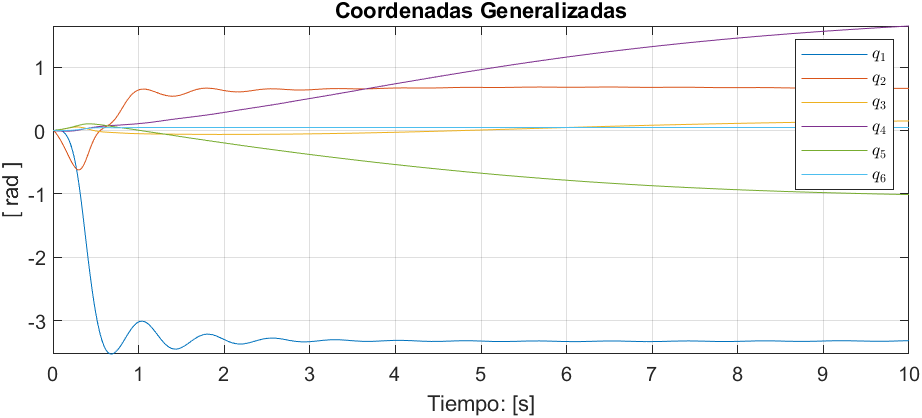
\includegraphics[scale=0.5]{coor_gen_caso_1.png} 
        \caption{Coordenadas Generalizadas Caso 1}
        \label{fig:CoordGenC1}
    \end{figure}

    \subsubsection{Energía Cinética}

    En el caso de la figura \ref{fig:eCinC1} identificamos un pico en la energía cinética a los 0.4 segundos y se estabiliza a partir del segundo 2, lo cual es consistente con lo esperado, puesto que se obserza una etapa de amortiguamiento y pérdida de energía, al alcanzar el equilibrio. Lo que significa que cuando se suelta el exoesqueleto de su posición de "CASA" y empieze a moverse como un péndulo, llegará un instante en que se detenga el movimiento ondulatorio, que es la fase de amortiguamiento que se observa.
    \begin{figure}[H]%[!ht]
            \centering
            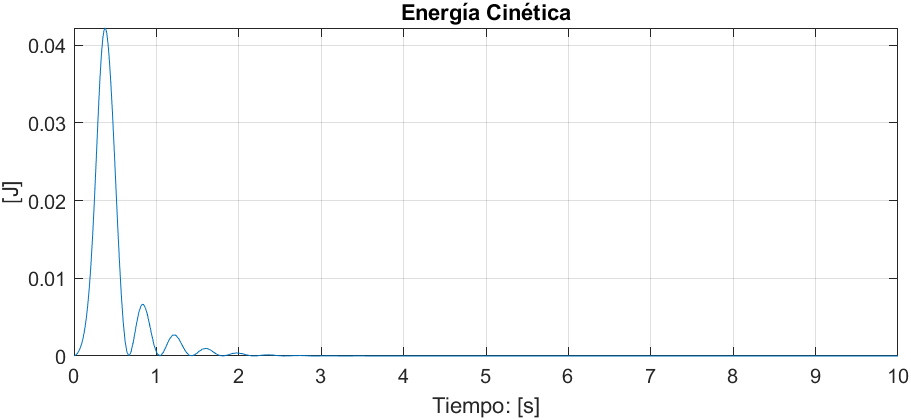
\includegraphics[scale=0.5]{ener_cin_caso_1.png} 
        \caption{Energía Cinética Caso 1}
        \label{fig:eCinC1}
    \end{figure}

    \subsubsection{Energía Potencial}
    La energía potencial inicia en 0.3 [J] y se puede observar en la figura \ref{fig:ePotC1} que a partir del segundo 2, se estabiliza al no tener movimiento el exoesqueleto y se aplica un offset en el "datum" para que no cause confusión en el usuario una energía negativa, sin embargo de no haberse implementado la constante arbitraria, hubiera tomado -0.3 [J] que sería el valor esperado en el instante que el exoesqueleto se queda estático.
    \begin{figure} [H]%[!ht]
            \centering
            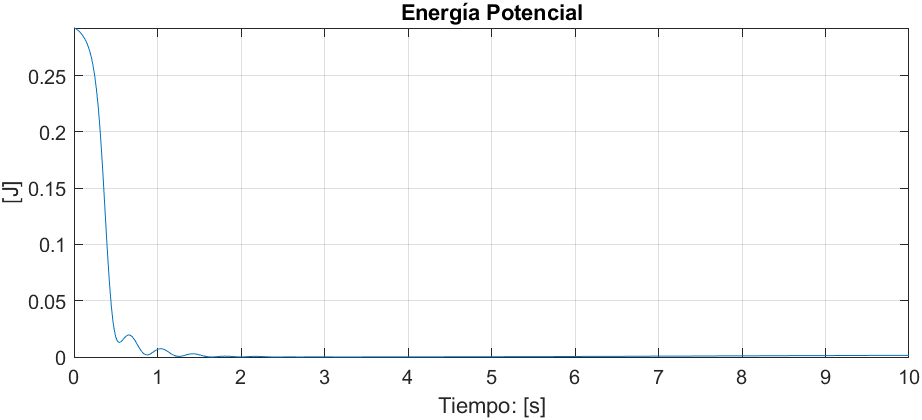
\includegraphics[scale=0.5]{ener_pot_caso_1.png} 
        \caption{Energía Potencial Caso 1}
        \label{fig:ePotC1}
    \end{figure}

    \subsubsection{Energía Mecánica}
    La energía mecánica es la suma de la energía cinética con la energía potencial; la gráfica \ref{fig:eMecC1} es muy parecida a la obtenida en \ref{fig:ePotC1} debido a que la energía cinética está en un rango muy pequeño con respecto a la potencial y por tanto casi no influye en la sumatoria. 

    \begin{figure} [H]%[!ht]
            \centering
            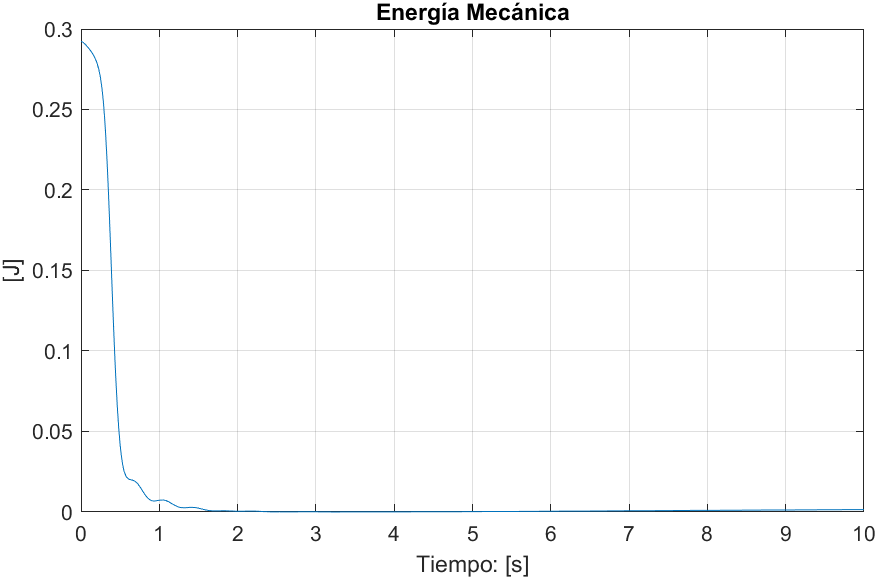
\includegraphics[scale=0.5]{ener_mec_caso_1.png} 
        \caption{Energía Mecánica Caso 1}
        \label{fig:eMecC1}
    \end{figure}

    \subsubsection{Velocidad Generalizada}
    La gráfica \ref{fig:VelGenC1}, nos muestra un cambio notable en la articulación del eslabón 1 y 2, mientras que el resto de los eslabones también tienen un efecto en su cambio de velocidad debido a que son parte de la cadena cinemática, sin embargo no son tan notorios porque el eje de la revoluta es perpendicular al eje donde se está llevando a cabo el movimiento de la primera articulación, que es justo lo que plasma la línea azul.

    \begin{figure}[H]% [!ht]
            \centering
            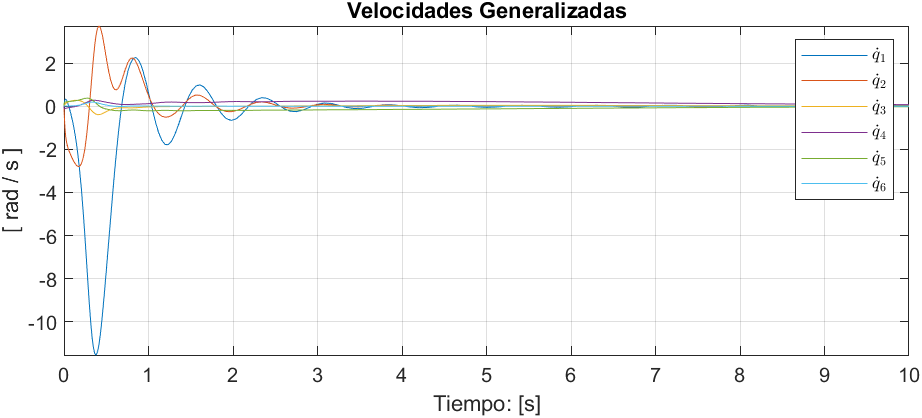
\includegraphics[scale=0.5]{vel_gen_caso_1.png} 
        \caption{Velocidad Generalizada Caso 1}
        \label{fig:VelGenC1}
    \end{figure}

\subsection{Caso 2}
    En el presente caso de estudio, se hicieron modificaciones en todos los parámetros (torque, factor de disipación y tiempo de simulación), los valores exactos se visualizan en la tabla \ref{ref:TablaC2}.
    \subsubsection{Parámetros} 

    \begin{table}[H]%[!ht]
        \centering
        \begin{center}
        \caption{Parámetros modificados del simulador (Sistema No Conservativo)} 
        \centering
        \bigskip
        \scalebox{0.7}{
            \begin{tabular}{c||cccccc|c}
            Parámetros & $\tau_1$ & $\tau_2$ & $\tau_3$ & $\tau_4$ & $\tau_5$ & $\tau_6$ & Unidades\\
            \hline
            Torques & -0.050 & 0.050 & -0.040 & -0.060 & 0.020 & 0.010 & [Nm] \\
            Factor de Disipación & \multicolumn{6}{c|}{0.006001} & [Ns/m] \\
            Tiempo de Simulación & \multicolumn{6}{c|}{20} & [s]\\
            \hline 
            \end{tabular}    }
        \end{center}
        \label{ref:TablaC2}
    \end{table}

    \subsubsection{Coordenadas Generalizadas}
    Las imágenes de la gráfica \ref{fig:CoordGenC2} son consistentes con los valores dados en los torques, puesto que las fuerza aplicadas en las articulaciones 1, 3 y 4 tienen valores negativos, esto significa que girarán en sentido opuesto a las manecillas del reloj, siguiendo la regla de la mano derecha, en oposición a las otras 3 articulaciones.

    \begin{figure} [H]%[!ht]
            \centering
            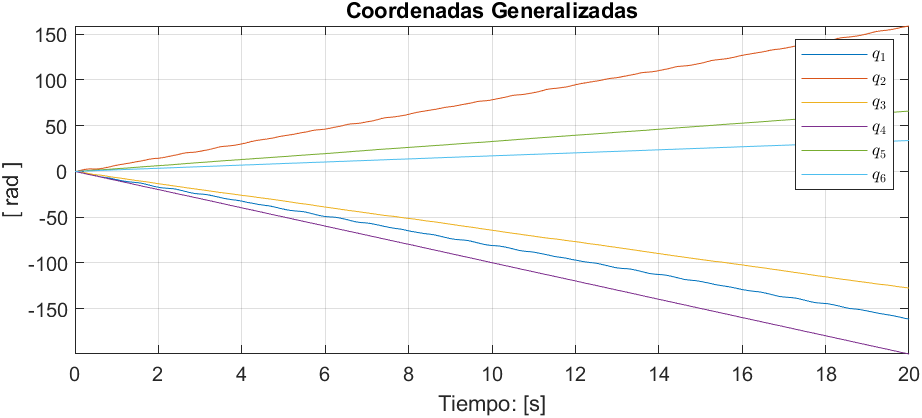
\includegraphics[scale=0.5]{coor_gen_caso_2.png} 
        \caption{Coordenadas Generalizadas Caso 2}
        \label{fig:CoordGenC2}
    \end{figure}

    \subsubsection{Energía Cinética}
    La gráfica \ref{fig:eCinC2} demuestra una función periódica, debido a que el torque ejercido en la articulación 1 es de 0.050 [Nm] y a pesar de que tiene la fuerza para dar una revolución completa, es importante remarcar que la fuerza es baja, eso significa que le está costando esfuerzo al motor, para ejercer la rotación completa y por este motivo observamos una ligera disminución en la energía cinética, que se incrementa rápidamente al pasar por el ángulo crítico, mismo que debe de estar entre 0 y $\pi/2$. 

    \begin{figure} [H]%[!ht]
            \centering
            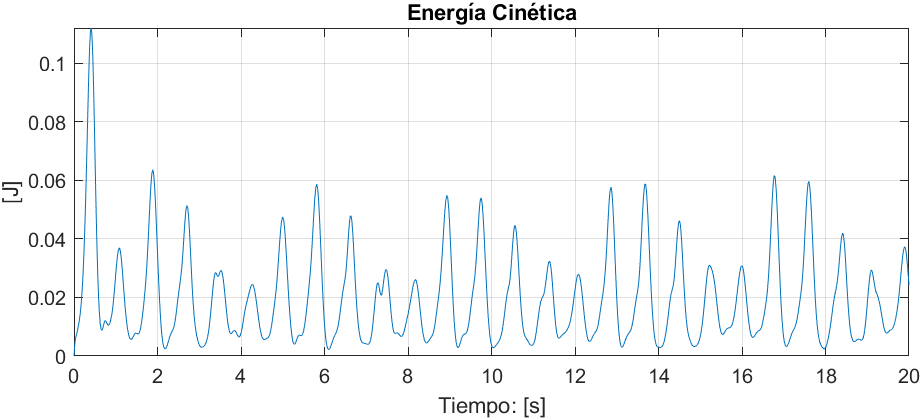
\includegraphics[scale=0.5]{ener_cin_caso_2.png} 
        \caption{Energía Cinética Caso 2}
        \label{fig:eCinC2}
    \end{figure}

    \subsubsection{Energía Potencial}
    La imagen obtenida por el osciloscopio, que se representa en la figura \ref{fig:ePotC2}  muestra la periodicidad del movimiento que está teniendo el exoesqueleto, algo importante a remarcar, es que está oscilando entre los valores de 0 y 2.2, pero nunca llega a los mismos 3 [J] de inicio, debido a que nunca se para completamente.

    \begin{figure} [H]%[!ht]
            \centering
            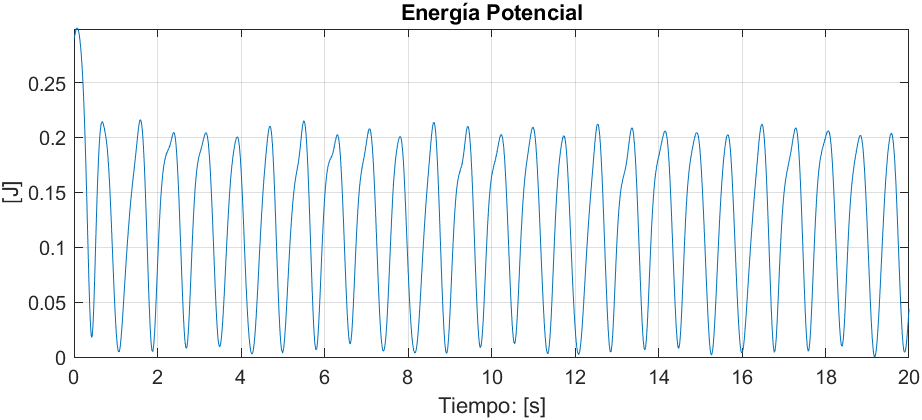
\includegraphics[scale=0.5]{ener_pot_caso_2.png} 
        \caption{Energía Potencial Caso 2}
        \label{fig:ePotC2}
    \end{figure}

    \subsubsection{Energía Mecánica}
    La gráfica de la figura \ref{fig:eMecC2} muestra un desfase positivo, proporcional a la magnitud de la energía cinética, con respecto de la gráfica de la figura \ref{fig:ePotC2}.
    \begin{figure} [H]%[!ht]
            \centering
            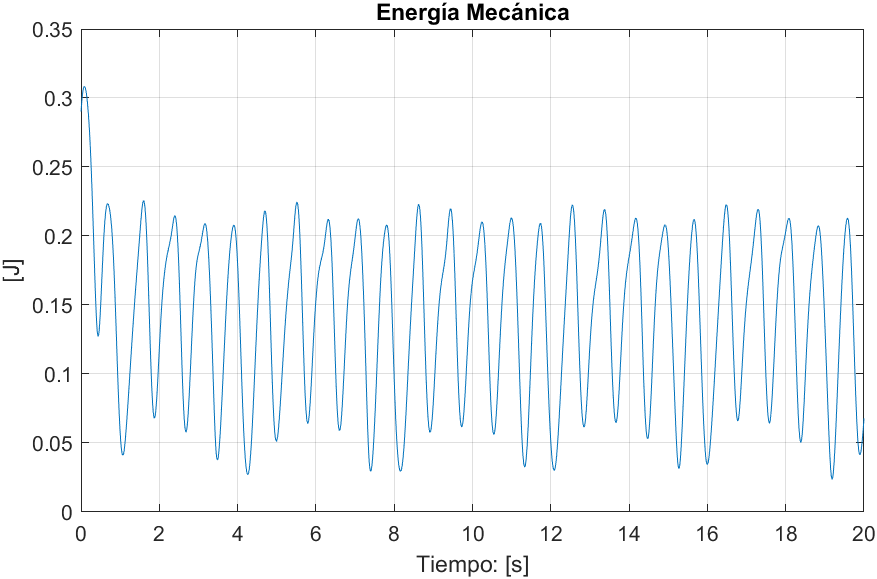
\includegraphics[scale=0.5]{ener_mec_caso_2.png} 
        \caption{Energía Mecánica Caso 2}
        \label{fig:eMecC2}
    \end{figure}

    \subsubsection{Velocidad Generalizada}
    Las articulaciones de los eslabones 1 y 2, en la gráfica \ref{fig:VelGenC2} son las que presentan variaciones con una mayor amplitud que el resto de las coordenadas generalizadas, además los referenciales $q_2$,$q_5$ y $q_6$ toman valores positivos y esto es consistente con los torques que fueron implementados y se visualizan en la tabla \ref{ref:TablaC2}.
    \begin{figure}[H]%[!ht]
            \centering
            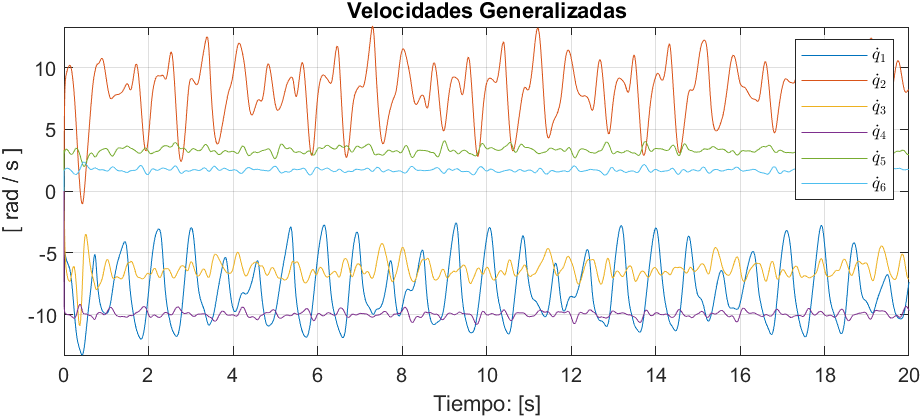
\includegraphics[scale=0.5]{vel_gen_caso_2.png} 
        \caption{Velocidad Generalizada Caso 2}
        \label{fig:VelGenC2}
    \end{figure}

\subsection{Caso 3}
    El último caso analizado representa un sistema conservativo, esto significa un acercamiento a un sistema ideal donde no hay disipación de energía, debido a que no se aplica una fuerza de fricción viscosa.

    \subsubsection{Parámetros}

    Los parámetros que se utilizaron para el caso 3, se ven reflejados en la tabla \ref{ref:TablaC3}, es decir, se están considerando nulos torques y sin fricción, así mismo se elongó el tiempo de simulación, para tener un mayor espacio de muestreo en el análisis.

    \begin{table}[H]%[!ht]
        \centering
        \begin{center}
        \caption{Parámetros modificados del simulador (Sistema Conservativo)} 
        \centering
        \bigskip
        \scalebox{0.7}{
            \begin{tabular}{c||cccccc|c}
            Parámetros & $\tau_1$ & $\tau_2$ & $\tau_3$ & $\tau_4$ & $\tau_5$ & $\tau_6$ & Unidades\\
            \hline
            Torques & 0 & 0 & 0 & 0 & 0 & 0 & [Nm] \\
            Factor de Disipación & \multicolumn{6}{c|}{0} & [Ns/m] \\
            Tiempo de Simulación & \multicolumn{6}{c|}{200} & [s]\\
            \hline 
            \end{tabular}    }
        \end{center}
        \label{ref:TablaC3}
    \end{table}

    \subsubsection{Coordenadas Generalizadas}

    La gráfica \ref{fig:CoordGenC3} muestra los cambios en la posición angular de cada una de las articulaciones a lo largo de 200 segundos simulados, se aprecia que el 6to referencial $q_6$ es el que más rotaciones presenta.

    \begin{figure} [H]% [!ht]
            \centering
            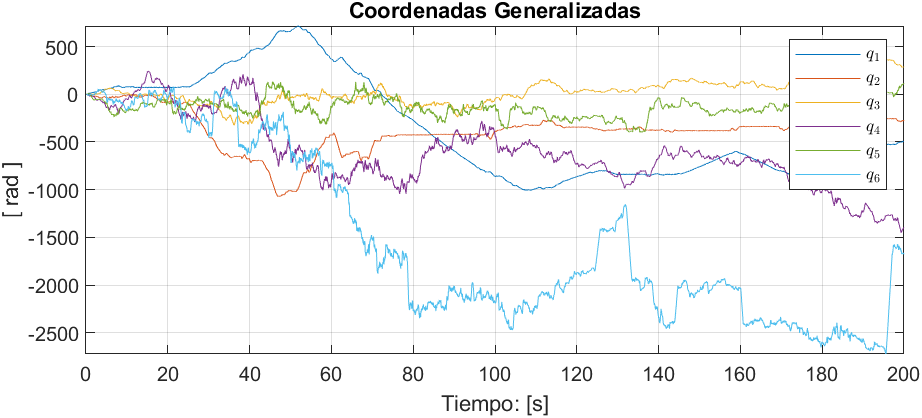
\includegraphics[scale=0.5]{coor_gen_caso_3.png} 
        \caption{Coordenadas Generalizadas Caso 3}
        \label{fig:CoordGenC3}
    \end{figure}

    \subsubsection{Energía Cinética}

    La energía cinética representada en la gráfica \ref{fig:eCinC3} muestra un pico a los 68 segundos, para finalmente tener un rango estable entre 0 y 1 Joule a partir de los 120 segundos. El rango 

    \begin{figure} [H]%[!ht]
            \centering
            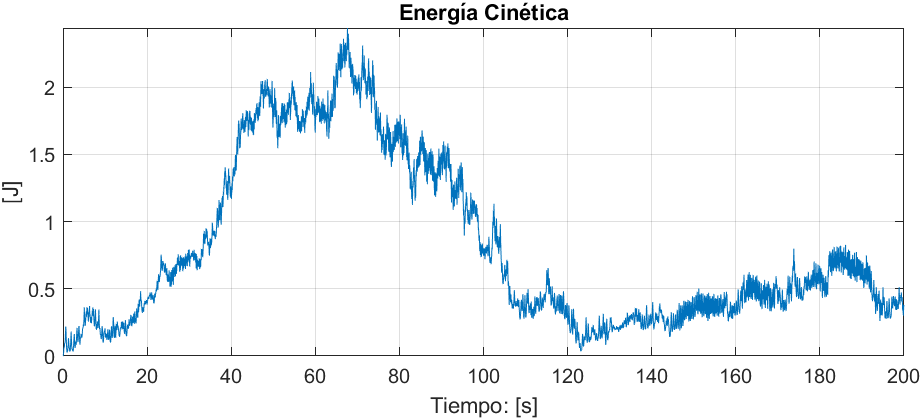
\includegraphics[scale=0.5]{ener_cin_caso_3.png} 
        \caption{Energía Cinética Caso 3}
        \label{fig:eCinC3}
    \end{figure}

    \subsubsection{Energía Potencial}

    La energía potencial es proporcional a la posición que tiene la cadena cinemática en función a un "datum", debido a lo anterior la gráfica \ref{fig:ePotC3} muestra que el exoesqueleto está tomando en promedio valores constantes y cercanos a cero, por eso su rango está entre 0 y 0.3 [J], porqué está teniendo una rotación en un movimiento perpetuo, al no haber fricción. 

    \begin{figure} [H]%[!ht]
            \centering
            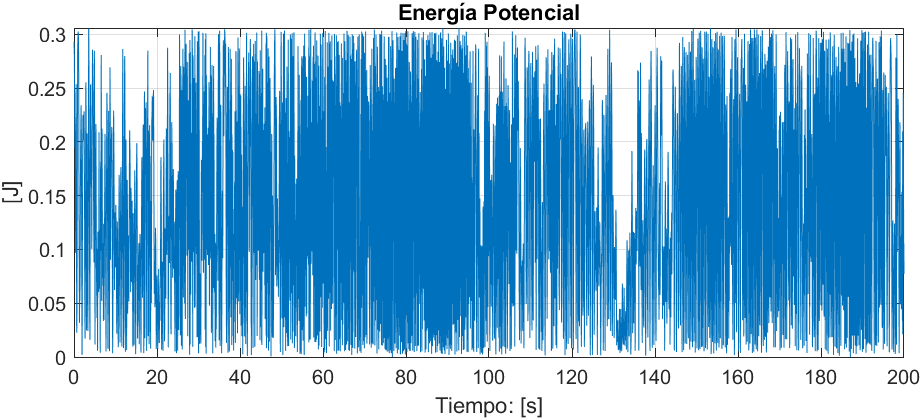
\includegraphics[scale=0.5]{ener_pot_caso_3.png} 
        \caption{Energía Potencial Caso 3}
        \label{fig:ePotC3}
    \end{figure}

    \subsubsection{Energía Mecánica}

    La gráfica \ref{fig:eMecC3} representa la energía mecánica total de un sistema conservativo, cuyo desfase positivo es de 0.3 [J], puesto que ese es el rango promedio máximo constante de la energía potencial. El pico que se observa en el lapso del tiempo de 0 a 68 segundos, refleja una inconsistencia a las leyes de la termodinámica, debido a que está reflejando creación de energía cinética, pues supera el rango máximo de la energía potencial.

    \begin{figure}[H]%[!ht]
            \centering
            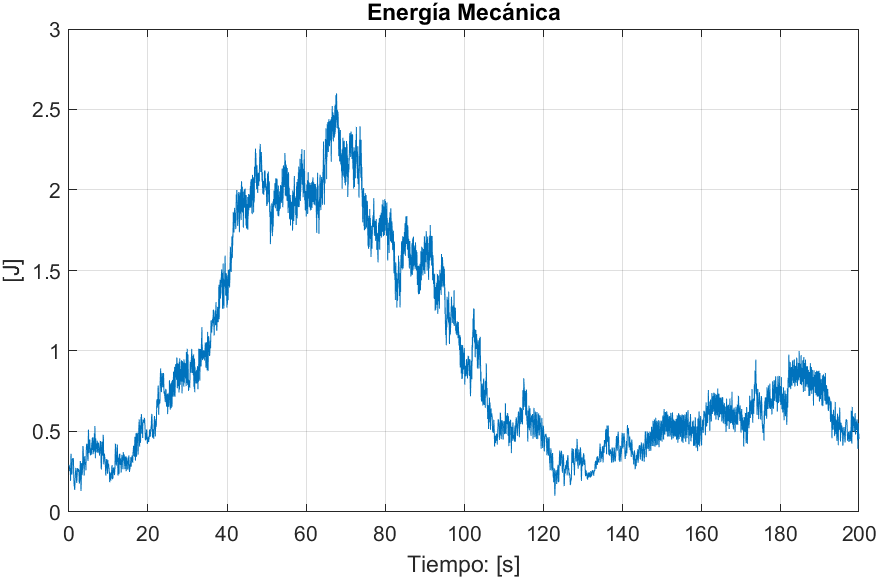
\includegraphics[scale=0.5]{ener_mec_caso_3.png} 
        \caption{Energía Mecánica Caso 3}
        \label{fig:eMecC3}
    \end{figure}

    \subsubsection{Velocidad Generalizada}

    La gráfica \ref{fig:VelGenC3} muestra en primer plano la velocidad generalizada del referencial $q_6$ en azul claro; de 0 a 40 segundos presenta una aceleración, alcanzando su punto máximo en el segundo 68, a partir de ese momento empieza a disminuir su velocidad, para finalmente estabilizar su velocidad en un rango de -1000 a 1000 rad/s, a partir de un tiempo de 120 segundos. 

    \begin{figure}[H]%[!ht]
            \centering
            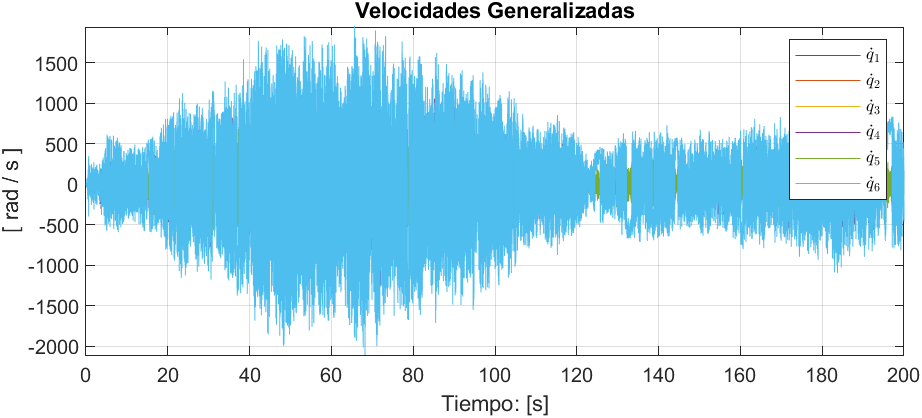
\includegraphics[scale=0.5]{vel_gen_caso_3.png} 
        \caption{Velocidad Generalizada Caso 3}
        \label{fig:VelGenC3}
    \end{figure}